We are also interested in the impacts of different traffic patterns on scaling
performance. As such, we send our test web server application web requests in a
variety of patterns and examine which traffic pattern the scaling method handles
well, and which traffic pattern the scaling method does not handle well.
Moreover, we also examine scaling methods in relation to each other with respect
to different traffic patterns, seeking to answer for which traffic patterns
predictive auto-scaling is beneficial and which traffic patterns predictive
auto-scaling is detrimental or meaningless.

In this thesis we examine two different traffic patterns that we feel are
fairly indicative of the different traffic patterns a web application may face.
We entitle these patterns \textit{increase-decrease}, and
\textit{flash-crowd}.\footnote{There are of course an infinite number of traffic
patterns that we could examine, and examining other options is an exciting
opportunity for future work.} We describe each of these patterns, and offer a
visual representation for each, below. Each pattern runs for forty minutes and makes
a maximum of 20 requests per second.\footnote{The actual traffic pattern takes
shape over 30 minutes, with five additional minutes of 1 request per second at
the start and end serving as a buffer.} These values were chosen to give
space for the lengthier pod initialization times and to keep the network from
becoming too congested respectively.

\begin{itemize}
  \item \textbf{increase-decrease}: The traffic pattern
    \textit{increase-decrease}, visible in Figure \ref{fig:increase-decrease},
    represents a web server facing constantly increasing and then constantly
    decreasing load. This scenario can be seen as representing for example, a
    restaurant in which people increasingly visit the site as it becomes closer
    and closer to a meal time, and decreasingly visit the site as a meal time
    becomes farther and farther away. After five minutes of initialization at
    1 request per second, our load
    generator builds from sending 1 request per second to 20 requests per
    second over the course of 15 minutes. After reaching the apex, the traffic
    generator then reduces from sending 30 requests per seconds to sending 1
    request per second, again over the course of 15 minutes.

    \begin{figure}[!h]
      \centerline{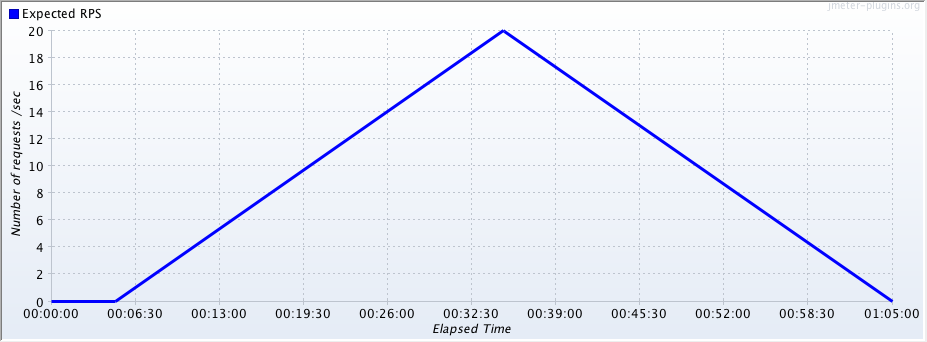
\includegraphics[scale=.4]{increase-decrease.jpg}}
      \caption{The increase-decrease Traffic Pattern}
      \label{fig:increase-decrease}
    \end{figure}

  \item \textbf{flash-crowd}: The traffic pattern \textit{flash-crowd}, visible
    in Figure \ref{fig:flash-crowd}, represents a web server facing a suddenly
    increasing, and then suddenly decreasing, amount of load. This scenario is
    indicative of, for example, a news website which will suddenly receive a
    short-lived burst of traffic when a major story hits. After five minutes of
    sending 1 request per second, our load generator
    slowly builds from sending 1 request per second
    to sending 5 requests per second, over the course of 11 minutes. Then, in
    just 4 minutes, our load generator jumps from sending 5 requests per second
    to sending 20 requests per second. After reaching the apex, the traffic
    generator decreases from sending 20 requests per second to sending 5
    requests per second, again in just 4 minutes. Finally, our load generator
    decreases from sending 5 requests per second to 1 request per second, over
    the course of 11 minutes.

    \begin{figure}[!h]
      \centerline{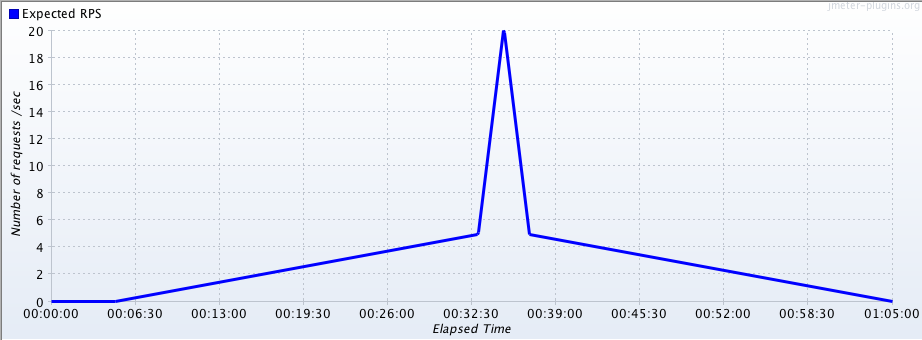
\includegraphics[scale=.4]{flash-crowd.jpg}}
      \caption{The flash-crowd Traffic Pattern}
      \label{fig:flash-crowd}
    \end{figure}

\end{itemize}
